\chapter{绪论}

\section{研究背景与概述}

核密度估计法(Kernel Density Estimation,KDE)是一种强大的非参数化数据估计方法,广泛应用于统计学、机器学习以及数据分析领域。不同于传统的参数化估计方法需要假设数据服从某种特定的概率分布(例如正态分布),并据此估计分布的参数(如均值和方差),核密度估计法能够直接从数据样本中推断出其概率密度函数,而无需对数据的分布形式做出任何假设。这种方法特别适用于那些难以用简单参数模型描述的数据集,因为它提供了更加灵活的方式来探索数据的内在结构。
非参数化的估计方法可以直接用于分析数据分布,检测热点,以及平滑数据~\cite{silverman_density_2018, gramacki_nonparametric_2018}。核密度估计法的应用十分广泛,例如金融风险预测~\cite{diebold_multivariate_1999, diebold_evaluating_1998, harvey_kernel_2012}、犯罪聚集分析~\cite{brunsdon_visualising_2007, nakaya_visualising_2010, hart_kernel_2014}和交通事故预防~\cite{black_highway_1991, xie_kernel_2008, plug_spatial_2011}。


核密度估计法通过对有限的离散数据集加权得到平滑的分布来估计其他位置的数据,即核密度。核密度的一般计算公式如下:
\begin{equation}
	F(q) = w \cdot \sum_{o_i \in O} {K}\Big(\frac{dist(q, o_i)}{b}\Big),
\end{equation}
其中,$q$ 是待查询核密度的位置;$F(q)$ 为查询点的核密度;$o_i \in O$ 是已知的数据点;$dist(q,o_i)$ 是查询点 $q$ 到数据点 $o_i$ 的距离,与带宽范围 $b$ 相除后得到归一化的距离;$K(\cdot)$ 是核函数,用于计算权重;$w$ 是放缩因子,用于将最后的结果变换到可视化范围(例如$0 \sim 255$)。

直观来看,核密度估计法是对数据点进行加权统计的一种方法,其基本思想是:对于每一个查询点,距离该查询点越近的数据点对最终的核密度估计贡献越大;反之,距离越远的数据点影响越小,当查询点与某个数据点之间的距离超过一定的带宽范围 $b$ 时,该数据点将不再对查询点处的核密度估计产生影响。

这种基于距离的权重分配方式具体是通过核函数来实现的。核函数是一类定义在 $[0, 1]$ 上的递减函数,它决定了不同距离下的权重分配规则,即决定了数据点在其邻域内的影响力分布。常见的核函数包括多项式核函数(例如三角核函数~\cite{fleuret_scale-invariance_2003, gong_estimating_2014},Epanechnikov核函数~\cite{samiuddin_nonparametric_1990, bil_identification_2013})和超越核函数(例如Gaussian核函数~\cite{scholkopf_comparing_1997, kristan_multivariate_2011},余弦核函数~\cite{de_felice_short-term_2015})。表~\ref{tab1} 总结了这些常见的核函数以及他们的表达式。

\begin{table}[!h]
	\centering
	\def\arraystretch{1.5}
	\caption{常见的核函数及其表达式}
	\label{tab1}
	\begin{tabular}{c|c}
		\hline
		核函数名称       & 核函数表示                                             \\ \hline \hline
		三角核函数 \cite{fleuret_scale-invariance_2003, gong_estimating_2014}   & $1-\frac{1}{b}dist(q,o_i)$         \\ 
		Epanechnikov核函数 \cite{samiuddin_nonparametric_1990, bil_identification_2013} & $1-\frac{1}{b^2}dist(q,o_i)^2$     \\ 
		Gaussian核函数 \cite{scholkopf_comparing_1997, kristan_multivariate_2011}     & $exp(-\frac{1}{b^2}dist(q,o_i)^2)$ \\ 
		余弦核函数 \cite{de_felice_short-term_2015}       & $\cos(\frac{1}{b}dist(q,o_i))$     \\ \hline
	\end{tabular}
\end{table}

不同的核函数会带来不同的核密度估计结果,因此选择合适的核函数对于准确描述数据分布至关重要。这些核函数的主要特点如下:
\begin{itemize}
	\item 三角核函数。这是一种简单的核函数,其形式为一个线性递减函数。当距离从0增加到带宽范围 $b$ 时,权重从1线性减少到0。三角核函数因其简单性和高效性,在许多场景中广泛应用。
	\item Epanechnikov核函数。这种核函数是一种二次多项式形式,其特点是在带宽范围内具有最优的均方误差性质。Epanechnikov核函数在接近带宽边界时迅速下降至零,使得核密度估计更加平滑。
	\item Gaussian核函数。这是最常用的核函数之一,基于高斯分布。它的特点是权重随距离呈指数衰减,即距离越远,权重下降得越快。Gaussian核函数在处理连续数据和平滑估计方面表现优异。
	\item 余弦核函数。这种核函数使用余弦函数来定义权重,其形式较为平滑,适用于需要更柔和过渡的应用场景。
\end{itemize}

核密度反映了带宽范围内数据点的综合影响,核函数会给较近的数据点赋予较高的权重,权重的大小由距离所决定,不同的距离度量方式会有不同的核密度估计结果。

目前,大部分算法均采用欧几里得距离作为距离度量的方法,欧几里得距离是一种直观且广泛应用的距离计算方法,它基于两点之间的直线距离,表明事件的影响随着直线传播。这种距离度量方式简单直接,适用于许多应用场景。然而,欧几里得距离的根号形式在计算中并不方便,如果不使用带有二次方形式的Epanechnikov核函数,很容易引入计算误差。相比之下,曼哈顿距离和切比雪夫距离则仅包含加减法和绝对值的运算,在计算形式上更加简单和高效。此外,还有一些更加复杂的距离度量方式,例如余弦相似度距离等,常常被应用在高维数据上。这些距离度量方式及其对应的距离函数如表~\ref{tab2}所示:

\begin{table}[!h]
	\centering
	\def\arraystretch{1.5}
	\caption{常见的距离度量方式及其表达式}
	\label{tab2}
	\begin{tabular}{c|c}
		\hline
		距离度量方式       & 距离函数表示   \\ \hline \hline
		欧几里得距离 & $d(x, y) = \sqrt{\sum{(x_i - y_i)}^2}$ \\ 
		曼哈顿距离   & $d(x, y) = \sum \vert x_i - y_i \vert$ \\ 
		切比雪夫距离 & $d(x, y) = \max \vert x_i - y_i \vert$ \\ 
		余弦相似度距离	 & $d(x, y) = \frac{x \cdot y}{\Vert x \Vert \cdot \Vert y \Vert}$     \\ \hline
	\end{tabular}
\end{table}

\section{现有工作与挑战}

由于核密度估计法易于理解、实现和可视化,它成为了许多地理信息系统软件中不可或缺的一部分,例如 ArcGIS~\cite{noauthor_arcgis_nodate},QGIS~\cite{noauthor_qgis_nodate}和KDV-Explorer~\cite{chan_kdv-explorer_2021}都支持这一算法。这些工具不仅提供了强大的数据分析能力,还允许用户通过直观的方式理解和展示数据的空间分布特征。然而,这些核密度估计法在以下三种场景中存在局限性:

\begin{figure}[t!]
	\centering
	\begin{subfigure}{0.4\linewidth}
		\centering
		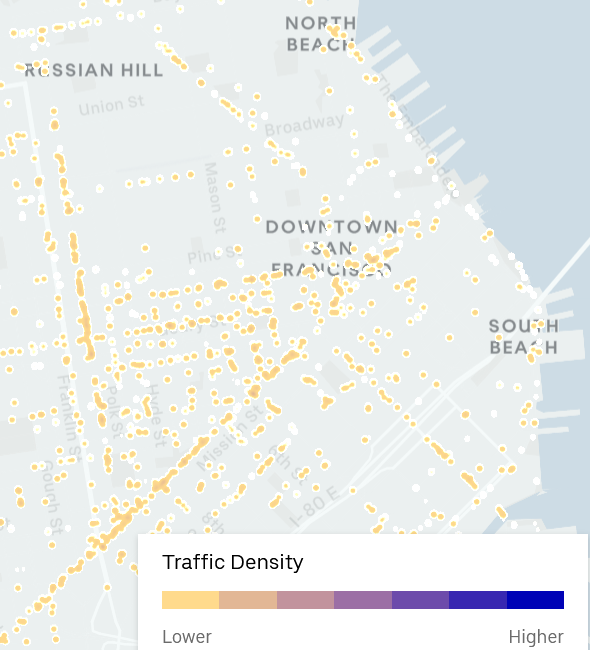
\includegraphics[width=0.8\linewidth]{figures/3a-6a-2020q1-RoadHeatmap-sanfrancisc.png}
		\caption{凌晨3点到6点的热力图}
		\label{subfig:morning_heatmap}
	\end{subfigure}
	\hspace{1em}
	\begin{subfigure}{0.4\linewidth}
		\centering
		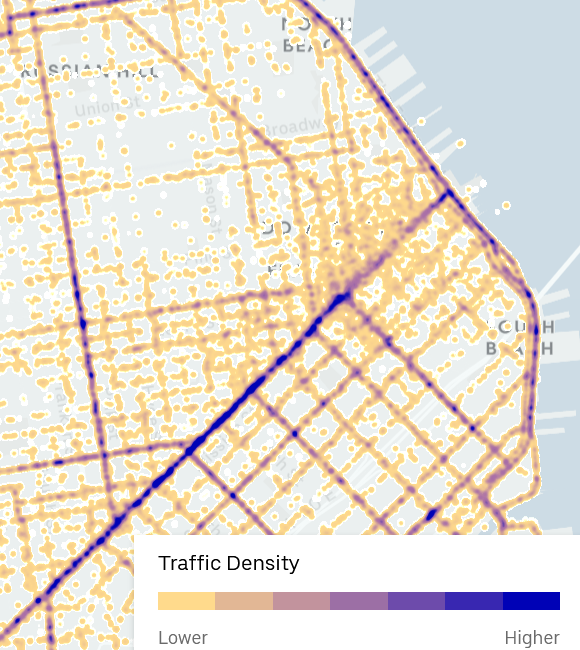
\includegraphics[width=0.8\linewidth]{figures/3p-6p-2020q1-RoadHeatmap-sanfrancisc.png}
		\caption{下午3点到6点的热力图}
		\label{subfig:afternoon_heatmap}
	\end{subfigure}
	\caption{不同时间窗口下的热力图对比。}
	\label{fig:temporal_heatmap}
\end{figure}

\begin{itemize}[leftmargin=*]

	\item 时间维度的聚类。核密度估计法是一种强大的工具,用于分析事件的空间分布,并通过空间距离(如欧几里得距离)来衡量事件的影响和计算核密度。然而,许多现实世界中的事件不仅在空间上相互关联,还与时间密切相关~\cite{black_highway_1991}。因此,单纯依赖空间距离进行KDE可能无法全面反映数据的真实特征。为了更准确地分析这些现象,我们需要将时间维度纳入考虑范围。
	
	具体来说,用户可能会选择过滤特定时间段内的事件,以揭示数据点在时间维度上的关联。~\cite{brunsdon_visualising_2007}。这种方法不仅可以帮助我们更好地理解事件的时间模式,还能为决策提供有价值的参考信息。例如,Uber Movement可以展示了特定时间段内的人口流动热图,如图~\ref{fig:temporal_heatmap}所示,这是2020年第一季度旧金山地区在凌晨3点到6点以及下午3点到6点两个不同时间段的交通流动性热图。可以很明显的看到下午3点到6点的流动性较高,且主干道的密度大于其他街道。这些密度较高的地区会更加拥堵,可以给后续的出租车派单和导航给出一定参考信息。
	
	\item 路网图的应用。一些研究发现,在路网图中采用欧几里得距离可能会高估核密度。图~\ref{fig:kde_example} 对比了平面核密度和网络核密度的计算方式(分别采用二维欧几里得距离和最短路径距离)。假设在查询点核数据点在平面上的距离为50米,如果我们使用欧几里得距离来计算这两个点之间的距离,那么核密度估计法会认为这两个点非常接近,并且会在它们之间分配较高的权重。然而,实际情况可能由于道路布局的原因,两点间的实际最短路径距离可能为70米。这意味着如果使用欧几里得距离进行核密度估计,该数据点的关联性会被高估,甚至会包含不应该存在的数据点。

	\item 多次在线查询。在实际应用中,用户往往需要根据不同的参数调用多次在线查询来生成一系列核密度估计值,并从中选取最符合需求的结果。参数的选择通常基于上一次的计算结果,这就要求多次实时查询而不仅仅是批次查询。这种动态调整和实时反馈的需求,使得传统的单次核密度估计方法难以满足现代数据分析的要求。然而,现有的工作主要关注于单次核密度估计的优化,缺少对多次在线查询的优化~\cite{gong_estimating_2014, gan_scalable_2017, plug_spatial_2011, brunsdon_visualising_2007, chan_safe_2021, cristianini_dynamically_1998, gramacki_nonparametric_2018}。
\end{itemize}

\begin{figure}[t!]
	\centering
	\begin{subfigure}{0.35\linewidth}
		\centering
		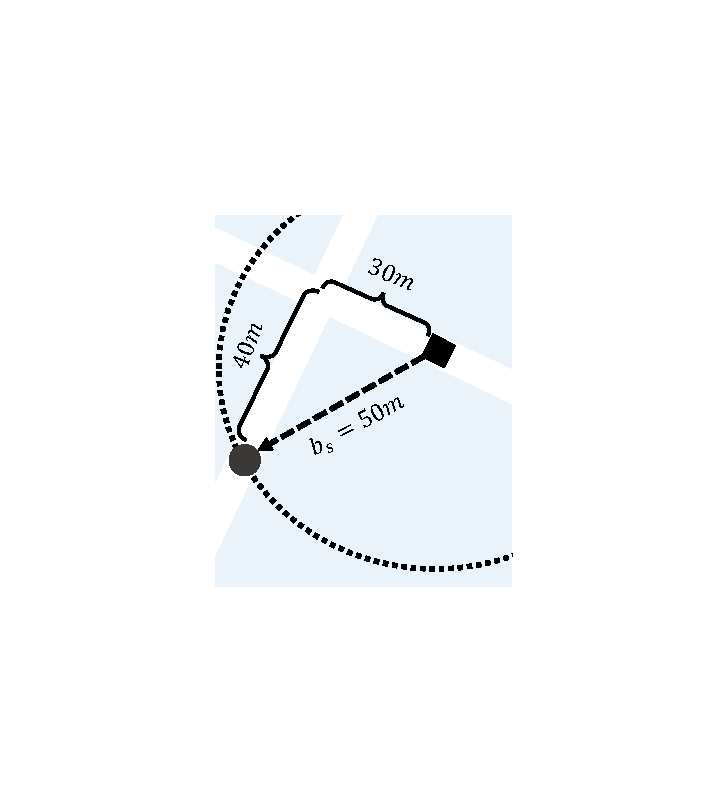
\includegraphics[width=0.8\linewidth]{figures/sec1_kde1.pdf}
		\caption{平面核密度估计}
		\label{subfig:loss_13}
	\end{subfigure}
	\hspace{1em}
	\begin{subfigure}{0.35\linewidth}
		\centering
		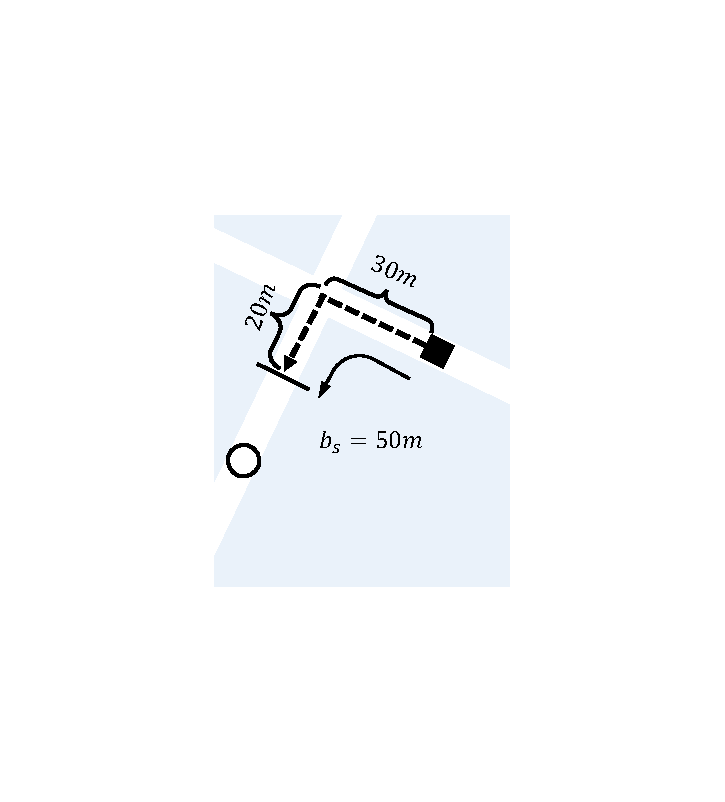
\includegraphics[width=0.8\linewidth]{figures/sec1_kde2.pdf}
		\caption{网络核密度估计}
		\label{subfig:loss_12}
	\end{subfigure}
	\caption{采用不同距离度量方式的核密度估计法的差异。平面核密度估计采用欧几里得距离,会低估查询点到数据点的距离,进而高估核密度。}
	\label{fig:kde_example}
\end{figure}

现有的工作在一定程度上已经能够优化核密度估计法,以解决上述问题。为了支持时间维度上的查询,一种常见的方式是根据固定的时间区间(如每小时、每天或每月)来逐个计算核密度~\cite{plug_spatial_2011},从而分析事件发生的时间模式及其关联性。这种方法允许我们观察特定时间段内的数据分布特征,并识别出潜在的趋势和规律。然而,这种方法虽然直观易懂,但在处理高分辨率时间序列时可能会面临计算效率的问题。
另一种常用方法是在三维时空中划分时空立方体~\cite{nakaya_visualising_2010, black_highway_1991}并利用时空核函数估计核密度\cite{brunsdon_visualising_2007, romano_visualizing_2017, chan_sws_2021},其本质是将时间视作另一个维度并进行划分。通过这种方式,不仅可以揭示事件在特定时间窗口内的空间分布,还能捕捉到它们随时间变化的动态特性。

针对路网图上的核密度估计,一个关键改进是使用最短路径距离代替传统的欧几里得距离。~\cite{borruso_network_2005},并沿边计算每个位置的核密度值,而不是在欧几里得空间中对每个像素进行计算~\cite{xie_kernel_2008}。这种方法更加符合实际的道路网络结构,避免了直线距离带来的误差。一些工作还进一步在在每条边上建立列表索引,来减少重复计算,实现更高效的核密度估计~\cite{chan_fast_2021}。这些改进通过优化数据结构和计算流程,显著提升了处理大规模路网数据的能力。


为了应对多次及在线查询的需求,传统的工作常采用基于分区的方法(例如K-d树~\cite{chan_efficient_2020, chan_quad_2020, chan_karl_2019}、网格化~\cite{hart_kernel_2014, black_highway_1991}、快速傅里叶变换(FFT)~\cite{silverman_algorithm_1982, gramacki_nonparametric_2018}、聚类~\cite{auber_interactive_2005, abello_ask-graphview_2006, hinneburg_denclue_2007}和分箱~\cite{liu_immens_2013, gramacki_nonparametric_2018, li_interactive_2014}等),这些方法的核心思想是将整个数据集分割成若干部分,并建立相应的数据结构,以便快速检索和聚合相邻的数据点,合并计算它们对核密度的贡献。\cite{liu_immens_2013}。

\section{研究贡献与创新}

尽管现有的研究在特定问题上进行了一些优化,如时间维度的查询、路网图上的核密度估计以及多次在线查询等,但目前仍缺乏一种单一的方法能够高效地解决所有这些主要挑战。因此,我们提出了针对时空数据集的时间网络核密度估计(Temporal Network Kernel Density Estimation,TN-KDE),旨在提供一个全面且高效的解决方案,以应对时空数据集中的复杂需求。

首先,我们提出了一种高效的算法,称为区间森林法(Range Forest Solution,RFS),用于高效计算任意时间窗口内的核密度。RFS采用了基于内存共享的树形索引来同时维护数据点的时间信息和位置信息。这种创新的数据结构能够在高效处理多个时间窗口查询的同时不增加额外的内存开销。

接着,我们还提出了动态区间森林法(Dynamic Range Forest Solution,DRFS),DRFS扩展了RFS,通过引入动态结构以支持插入操作。DRFS还为用户提供了不同等级的量化参数,以达到不同的计算精度。这种灵活的设计允许用户的根据实际需求和限制来动态调整索引的大小,便于用户平衡输出结果的精度和计算时间的开销。

更进一步,我们还注意到相邻查询点的核密度值往往是平滑变化的,且共享了大量相似的计算步骤。针对这一现象,我们设计了一种叫做线段点共享(Lixel Sharing,LS)的技术,允许将相似的计算结果共享到多个查询点上。

最后,我们的框架支持更复杂的核函数,包括指数核函数和余弦核函数,且能够计算精确的核密度。

此外,考虑到TN-KDE中会频繁调用最短路径算法的需求,为了提高计算效率和处理大规模数据集的能力,我们还探索了如何将最短路径算法扩展到分布式环境中计算。我们简单介绍了传统图算法是如何移植到分布式环境下,以及相关的底层设计(包括图划分算法和图计算模式),然后给出了常见图计算平台上的分布式最短路径算法的实现,同时对这些代码进行运行时间和扩展性的评估,给出性能对比和选取参考。

本论文的主要贡献安排如下:

\begin{itemize}[leftmargin=*]
	\item 在第\ref{sec3:preliminaries}章中,我们正式地定义了空间网络核密度估计(TN-KDE)问题,并介绍了一个基础框架。
	
	\item 在第\ref{sec5:solution}章和第\ref{sec7:dynamic}章中,我们分别介绍了两种算法区间森林法(RFS)和动态区间森林法(DRFS),用于高效地计算空间网络核密度,以及所支持的插入操作。
	
	\item 在第\ref{sec6:LixelsAggregaion}章中,我们提出了线段点共享(LS)的优化技术,以减少冗余计算并提高效率。同时在第\ref{sec7:kernel}章中,我们分析了许多可以应用于我们框架的非多项式核函数。
	
	\item 在第\ref{sec8:exp}章中,通过对不同规模和类别的真实世界数据集进行测试,展示了我们提出方法的高效性和有效性。
	
	\item 在第\ref{sec:distribution1}章中,我们介绍了分布式图计算的相关背景,包括图计算的划分算法和图计算的计算模式,并给出了几个常见的计算平台及这些计算平台上的最短路径算法实现。
	
	\item 在第\ref{sec:distribution2}章中,我们对这些最短路径算法在不同的计算资源配置下进行测试,主要包括运行时间和扩展性,给出了这些平台的性能对比和选取参考。
\end{itemize}
